\chapter{Zestaw 6, System.Windows.Forms}

\begin{flushright}
Liczba punkt�w do zdobycia: {\bf 6/50}
\end{flushright}

\begin{enumerate}
  
\item ({\bf 2p}) Napisa� program, kt�ry odtworzy nast�puj�cy wygl�d okna z rysunku \ref{r1}.
\label{okno_dialogowe}

	\begin{figure}
	\begin{center}
	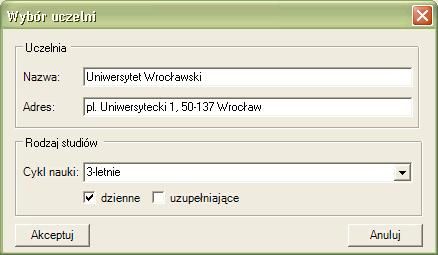
\includegraphics[width=0.75\textwidth]{z1_01}
	\end{center}
	\caption{Wygl�d okna do zadania [\ref{okno_dialogowe}]}
	\label{r1}
	\end{figure}

      Okno zawiera dwie ramki grupuj�ce ({\em GroupBox}). Pierwsza ramka zawiera dwa pola tekstowe
      ({\em TextBox}), druga zawiera pole wyboru ({\em ComboBox}) oraz dwa przyciski stanu ({\em CheckBox}).

      Lista rozwijalna pola wyboru powinna by� wype�niona przyk�adowymi nazwami.

      Po wybraniu przez u�ytkownika przycisku {\bf Akceptuj}, wyb�r powinien zosta� zaprezentowany w oknie
      informacyjnym (rysunek \ref{r2}).

      	\begin{figure}
	\begin{center}
	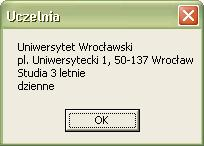
\includegraphics[width=0.25\textwidth]{z1_02}
	\end{center}
	\caption{Informacja dla u�ytkownika do zadania [\ref{okno_dialogowe}]}
	\label{r2}
	\end{figure}

      Naci�ni�cie przycisku {\bf Anuluj} powinno zako�czy� program.
      
      {\em Uwaga! Komunikat w oknie informacyjnym zale�y oczywi�cie od
      danych wprowadzonych przez u�ytkownika na formularzu g��wnym}
  
\item ({\bf 2p}) Napisa� program, kt�ry zademonstruje dzia�anie nast�puj�cych formant�w biblioteki standardowej
\begin{itemize}
\item {\bf MenuStrip}
\item {\bf ContextMenuStrip}
\item {\bf ToolStrip}
\item {\bf ToolTip}
\item {\bf TabControl}
\item {\bf SplitContainer}
\item {\bf Panel}
\item {\bf FlowLayoutPanel}
\end{itemize}
        
\item ({\bf 1p}) Napisa� program, kt�ry zademonstruje dzia�anie nast�puj�cych formant�w biblioteki standardowej
\begin{itemize}
\item {\bf OpenFileDialog}
\item {\bf SaveFileDialog}
\item {\bf FolderBrowserDialog}
\end{itemize}

\item ({\bf 1p}) Pokaza� jak w aplikacji korzysta� z pliku konfiguracyjnego aplikacji - do pliku konfiguracyjnego zapisa� parametry typu {\bf string} (litera�),
{\bf int} (liczba) oraz {\bf bool} (warto�� logiczna) a w aplikacji poprawnie je odczyta� i pokaza� warto�ci.
  
\end{enumerate}

